\section{Experiments}
\label{sec:experiments}
This section presents quantitative \& qualitative experiments on event de-flaring.

\subsection{Experimental Settings}

Our proposed model is trained exclusively on \emph{E-Flare2.7K-train}, and tested on \emph{E-Flare2.7K-test}, \emph{E-Flare-R}, and \emph{DSEC-Flare} datasets, respectively.


\noindent\textbf{Baselines.}
Image-based flare removal methods~\cite{wu2021train,dai2022flare7k,dai2024flare7k++,zhou2023improving} are not directly applicable to event streams, as they operate on dense pixel frames; adapting them would require a non-trivial domain translation that is itself an open problem. We instead compare against five representative baselines: (1) the unprocessed \emph{RAW Input}; (2) \emph{Voxel Transform}, a round-trip codec baseline that encodes events into voxel grids and decodes them back without any learned processing, isolating the effect of the representation itself; (3) \emph{EFR}~\cite{wang2022linear}, a classical flicker-removal filter; and (4–5) two recent denoising variants from~\cite{shi2024polarity}: \emph{PFD-A} (general noise suppression) and \emph{PFD-B} (light-interference mitigation). Due to space limitations, more details are provided in the \textbf{Appendix}.


\noindent\textbf{Evaluation Protocol.} 
As no established metrics exist for this task, we adapt measures from related event-based studies.  
For \textbf{event-level} fidelity, inspired by PECS~\cite{han2024physical}, we design two metrics: the \emph{Chamfer Distance} ($\downarrow$), the average nearest-neighbor distance to ground-truth events; and the \emph{Gaussian Distance} ($\downarrow$), applying Gaussian weighting to suppress outliers. For \textbf{voxel-level} structural quality, we adopt the standard evaluation suite from V2CE~\cite{zhang2023v2ce}, including \emph{Mean Squared Error} (MSE, $\downarrow$), \emph{Pooled MSE} (PMSE, $\downarrow$), and \emph{Binarized-Grid F1} scores (R-F1, T-F1, TP-F1, all $\uparrow$) to jointly and comprehensively capture reconstruction accuracy and overall precision-recall balance.


\noindent\textbf{Implementation Details.} 
Our model is trained on \textbf{E-Flare2.7K} for $40$k iterations on a single NVIDIA RTX $3090$ GPU. The network employs a standard residual 3D U-Net, demonstrating that our physically grounded data alone suffice for effective learning. Due to space limitations, more implementation details have been provided in the \textbf{Appendix}.





\begin{table*}[t]
    \centering
    \caption{\textbf{Quantitative comparisons on the E-Flare2.7K test set}. We evaluate against five event-based de-flaring baselines using event-level and voxel-level metrics, respectively. Cell backgrounds highlight the \colorbox{gray!20}{raw baseline}, \colorbox{ev_red!20}{second-best}, and \colorbox{ev_blue!20}{best} value per metric. The final row shows the percentage improvement of our method over the second-best ($\downarrow$: lower is better, $\uparrow$: higher is better). Ch. = Chamfer Distance; Gau. = Gaussian Distance; PM2/PM4 = Pooled MSE at scales 2/4.}
    \vspace{-0.3cm}
    \label{tab:main_sim_quant}
    \small
    \resizebox{\textwidth}{!}{
    \begin{tabular}{lcccccccc}
    \toprule
    \textbf{Method} & ~~~Ch.$\downarrow$~~~ & ~~~Gau.$\downarrow$~~~ & ~~MSE$\downarrow$~~ & ~~PM2$\downarrow$~~ & ~~PM4$\downarrow$~~ & ~~R-F1$\uparrow$~~ & ~~T-F1$\uparrow$~~ & ~~TP-F1$\uparrow$~~
    \\
    \midrule
    \textcolor{gray}{$\bullet$}~\textcolor{gray}{Raw Input} & \cellcolor{gray!20}\textcolor{gray}{$1.3555$} & \cellcolor{gray!20}\textcolor{gray}{$0.5222$} & \cellcolor{gray!20}\textcolor{gray}{$0.8315$} & \cellcolor{gray!20}\textcolor{gray}{$0.3666$} & \cellcolor{gray!20}\textcolor{gray}{$0.3430$} & \cellcolor{gray!20}\textcolor{gray}{$0.5138$} & \cellcolor{gray!20}\textcolor{gray}{$0.6303$} & \cellcolor{gray!20}\textcolor{gray}{$0.6939$}
    \\
    \textcolor{ev_red}{$\bullet$}~EFR \cite{wang2022linear} & $1.3237$ & $0.5439$ & $0.5357$ & $0.2019$ & $0.1755$ & $0.1616$ & $0.3572$ & $0.4811$
    \\
    \textcolor{ev_red}{$\bullet$}~PFD-A \cite{shi2024polarity} & $1.3958$ & $0.5397$ & $0.8357$ & $0.3637$ & $0.3392$ & $0.4383$ & \cellcolor{ev_red!20}$0.5496$ & $0.6125$ 
    \\
    \textcolor{ev_red}{$\bullet$}~PFD-B \cite{shi2024polarity} & \cellcolor{ev_red!20}$1.2496$ & \cellcolor{ev_red!20}$0.4613$ & \cellcolor{ev_red!20}$0.2851$ & $0.1159$ & $0.1021$ & \cellcolor{ev_red!20}$0.4460$ & $0.5155$ & $0.5727$ 
    \\
    \textcolor{ev_red}{$\bullet$}~Voxel Transform & $1.2923$ & $0.5576$ & $0.3495$ & \cellcolor{ev_red!20}$0.1037$ & \cellcolor{ev_red!20}$0.0829$ & $0.2177$ & $0.5444$ & \cellcolor{ev_red!20}$0.6318$ 
    \\
    \midrule
    \textcolor{ev_blue}{$\bullet$}~\ours & \cellcolor{ev_blue!20}$\mathbf{0.4477}$ & \cellcolor{ev_blue!20}$\mathbf{0.2646}$ & \cellcolor{ev_blue!20}$\mathbf{0.1269}$ & \cellcolor{ev_blue!20}$\mathbf{0.0487}$ & \cellcolor{ev_blue!20}$\mathbf{0.0435}$ & \cellcolor{ev_blue!20}$\mathbf{0.7071}$ & \cellcolor{ev_blue!20}$\mathbf{0.7627}$ & \cellcolor{ev_blue!20}$\mathbf{0.7794}$ 
    \\
    \emph{Improvement (\%)} $\uparrow$ & $64.2\%$$\uparrow$ & $42.6\%$$\uparrow$ & $55.5\%$$\uparrow$ & $53.0\%$$\uparrow$ & $47.5\%$$\uparrow$ & $58.5\%$$\uparrow$ & $38.8\%$$\uparrow$ & $23.4\%$$\uparrow$
    \\
    \bottomrule
    \end{tabular}}
    \vspace{-0.3cm}
\end{table*}


\begin{figure*}[t]
    \centering
    \includegraphics[width=\textwidth]{figures/simu_R.pdf}
    \vspace{-0.6cm}
    \caption{\textbf{Qualitative assessments on E-Flare2.7K}. Each column shows the output of a different method applied to the same flare-corrupted input. The rightmost column displays the ground truth for reference. Best viewed in color and zoomed-in for details.}
    \label{fig:qualitative_sim}
    \vspace{-0.2cm}
\end{figure*}




\subsection{Main Results}
\label{sec:main_results}

% \noindent\textbf{Evaluation on Simulated Data.}
% Table~\ref{tab:main_sim_quant} reports quantitative results on our simulated test set. Existing methods prove fundamentally inadequate for event-based de-flaring. While some baselines can suppress strong light sources, their rule-based filtering fails to distinguish structured flare patterns from legitimate events, often removing valid signals. In contrast, our learning-based model effectively captures the non-local and spatio-temporal characteristics of lens flare. This is evidenced by its commanding performance, achieving, for instance, a $\mathbf{64.2\%}$ improvement in Chamfer distance and a $\mathbf{55.5\%}$ reduction in MSE over the next-best method. This clear superiority across all metrics underscores its ability to selectively remove artifacts while preserving authentic scene dynamics.
\noindent\textbf{Evaluation on Simulated Data.}
Table~\ref{tab:main_sim_quant} shows that existing methods are ill-suited for event-based de-flaring. Their rule-based filtering fails to distinguish structured flare patterns from legitimate events, often removing valid signals. In contrast, our learning-based model effectively captures the flare's non-local, spatio-temporal characteristics, enabling it to selectively remove artifacts while preserving scene dynamics. This yields, for instance, a $\mathbf{64.2\%}$ improvement in Chamfer distance and a $\mathbf{55.5\%}$ improvement in MSE over the next-best method.

\begin{table*}[t]
    \centering
    \caption{\textbf{Quantitative comparisons on the E-Flare-R dataset}. We evaluate against five event-based de-flaring baselines using event-level and voxel-level metrics, respectively. Cell backgrounds highlight the \colorbox{gray!20}{raw baseline}, \colorbox{ev_red!20}{second-best}, and \colorbox{ev_blue!20}{best} value per metric. The final row shows the percentage improvement of our method over the second-best ($\downarrow$: lower is better, $\uparrow$: higher is better). Ch. = Chamfer Distance; Gau. = Gaussian Distance; PM2/PM4 = Pooled MSE at scales 2/4.}
    \vspace{-0.3cm}
    \label{tab:main_real_quant}
    \small
    \resizebox{\textwidth}{!}{
    \begin{tabular}{lcccccccc}
    \toprule
    \textbf{Method} & ~~~Ch.$\downarrow$~~~ & ~~~Gau.$\downarrow$~~~ & ~~MSE$\downarrow$~~ & ~~PM2$\downarrow$~~ & ~~PM4$\downarrow$~~ & ~~R-F1$\uparrow$~~ & ~~T-F1$\uparrow$~~ & ~~TP-F1$\uparrow$~~
    \\
    \midrule
    \textcolor{gray}{$\bullet$}~\textcolor{gray}{Raw Input} & \cellcolor{gray!20}\textcolor{gray}{$1.7855$} & \cellcolor{gray!20}\textcolor{gray}{$0.7170$} & \cellcolor{gray!20}\textcolor{gray}{$0.8158$} & \cellcolor{gray!20}\textcolor{gray}{$0.3431$} & \cellcolor{gray!20}\textcolor{gray}{$0.3266$} & \cellcolor{gray!20}\textcolor{gray}{$0.2299$} & \cellcolor{gray!20}\textcolor{gray}{$0.2915$} & \cellcolor{gray!20}\textcolor{gray}{$0.3093$}
    \\
    \textcolor{ev_red}{$\bullet$}~EFR \cite{wang2022linear} & $1.8191$ & $0.7266$ & $0.3388$ & $0.1403$ & $0.1330$ & $0.0839$ & $0.1807$ & $0.2372$ 
    \\
    \textcolor{ev_red}{$\bullet$}~PFD-A \cite{shi2024polarity} & \cellcolor{ev_red!20}$1.7642$ & \cellcolor{ev_red!20}$0.7067$ & $0.7924$ & $0.3341$ & $0.3182$ & \cellcolor{ev_red!20}$0.2386$ & \cellcolor{ev_red!20}$0.3081$ & \cellcolor{ev_red!20}$0.3283$
    \\
    \textcolor{ev_red}{$\bullet$}~PFD-B \cite{shi2024polarity} & $2.0838$ & $0.8504$ & \cellcolor{ev_red!20}$0.2759$ & $0.1121$ & $0.1049 $& $0.0300$ & $0.0717$ & $0.0880$ 
    \\
    \textcolor{ev_red}{$\bullet$}~Voxel Transform & $1.9535$ & $0.8167$ & $0.3140$ & \cellcolor{ev_red!20}$0.0964$ & \cellcolor{ev_red!20}$0.0836$ & $0.1036$ & $0.2729$ & $0.3255$ 
    \\
    \midrule
    \textcolor{ev_blue}{$\bullet$}~\ours & \cellcolor{ev_blue!20}$\mathbf{1.1368}$ & \cellcolor{ev_blue!20}$\mathbf{0.4651}$ & \cellcolor{ev_blue!20}$\mathbf{0.1741}$ & \cellcolor{ev_blue!20}$\mathbf{0.0690}$ & \cellcolor{ev_blue!20}$\mathbf{0.0644}$ & \cellcolor{ev_blue!20}$\mathbf{0.3498}$ & \cellcolor{ev_blue!20}$\mathbf{0.3386}$ & \cellcolor{ev_blue!20}$\mathbf{0.3011}$
    \\
    \emph{Improvement (\%)} $\uparrow$ & $35.6\%$$\uparrow$ & $34.2\%$$\uparrow$ & $36.9\%$$\uparrow$ & $28.4\%$$\uparrow$ & $23.0\%$$\uparrow$ & $46.6\%$$\uparrow$ & $9.9\%$$\uparrow$ & -$8.3\%$$\downarrow$
    \\
    \bottomrule
    \end{tabular}}
    \vspace{-0.3cm}
\end{table*}


\begin{figure*}[t]
    \centering
    \includegraphics[width=\textwidth]{figures/real_R.pdf}
    \vspace{-0.6cm}
    \caption{\textbf{Qualitative assessments on E-Flare-R.}  Each column shows the output of a different method applied to the same flare-corrupted input. The rightmost column displays the ground truth for reference. Best viewed in color and zoomed-in for details.}
    \label{fig:qualitative_real}
    \vspace{-0.2cm}
\end{figure*}


% \noindent\textbf{Evaluation on Paired Real-World Data.}
% To assess real-world generalization, we evaluate the model on our challenging paired dataset. The network is trained \emph{solely} on simulated data, making this a zero-shot sim-to-real evaluation. As shown in Table~\ref{tab:main_real_quant}, the performance trends largely remain consistent. \textbf{E-DeflareNet} significantly outperforms all baselines in most key metrics, such as a $\mathbf{35.6\%}$ improvement in Chamfer distance and a $\mathbf{34.2\%}$ improvement in Gaussian distance over the second-best method. 
% While TP-F1 shows a slight decrease ($-8.3\%$), this reflects a conservative denoising strategy that prioritizes avoiding the introduction of false events over aggressively recovering every noisy one. This focus on high fidelity is precisely why our method excels on stricter metrics like Chamfer, Gaussian, and R-F1, which more heavily penalize structural distortions and false positives. The strong overall performance demonstrates both the robustness of our model and the effectiveness of our simulation pipeline.
\noindent\textbf{Evaluation on Paired Real-World Data.}
Our model, trained \emph{solely} on simulated data, generalizes zero-shot to real-world data. Table~\ref{tab:main_real_quant} shows consistent performance trends. \textbf{E-DeflareNet} significantly outperforms all baselines on most key metrics, such as $\mathbf{35.6\%}$ in Chamfer distance. While TP-F1 shows a slight decrease (-$8.3\%$), this reflects a conservative strategy that prioritizes high fidelity by avoiding false positives over aggressively recovering every noisy event. This trade-off yields superior results on stricter metrics like Chamfer and R-F1. Overall, these results validate model robustness and pipeline effectiveness.


\noindent\textbf{Qualitative Analysis.}
Figs.~\ref{fig:qualitative_sim}--\ref{fig:qualitative_real} further confirm these findings. Baselines tend to leave substantial flare artifacts or excessively suppress light sources, compromising scene integrity. In contrast, \textbf{E-DeflareNet} cleanly removes structured flare while preserving illumination consistent with ground truth, recovering physically plausible event streams with high spatial and temporal fidelity.




\subsection{Ablation Study}
\label{sec:ablation}

We ablate three design variants on E-Flare-R (Table~\ref{tab:ablation_main}):
\textbf{(1)} \emph{No Light}: ground truth incorrectly removes the light source, treating de-flaring as complete elimination;
\textbf{(2)} \emph{Simple}: direct additive fusion, ignoring irradiance superposition physics;
\textbf{(3)} \emph{Full Model (Ours)}: physics-guided synthesis with probabilistic non-linear event suppression (PNL-ES) as described above.
% \textbf{(4)} \emph{Full Model + Jitter}: our method with additional temporal jitter augmentation to test whether gains stem from physical modeling or stochastic augmentation.

The results reveal a clear performance hierarchy.
First, the catastrophic failure of \emph{No Light} (Chamfer: $1.9745$ \vs $1.1368$ for ours) confirms that \textbf{preserving the actual light source in ground truth is essential}. This variant treats all flare-related events as noise to be removed, destroying semantically valid illumination.
Second, the substantial gap between \emph{Simple} and our \emph{Full Model} (Chamfer: $1.3434$ \vs $1.1368$, a $15.4\%$ improvement) validates the necessity of \textbf{physics-guided event fusion}. The simple additive approach implicitly sets $w_{\mathrm{bg}} = 1$ regardless of relative irradiance, ignoring the physical weighting derived in Sec.~\ref{ssec:forward_model}. This is especially damaging in flare-dominated regions where $w_{\mathrm{bg}} \to 0$: it erroneously preserves all background events that the real sensor would suppress, training the network on physically implausible data.
% Third, and crucially, the performance drop in \emph{Full Model + Jitter} (Chamfer: $1.6811$ \vs $1.1368$, a $47.9\%$ degradation) demonstrates that \textbf{our gains arise from physical insight, not data augmentation}. The temporal jitter severs the strict spatio-temporal correspondence between each event and its physical weight $w_{\mathrm{bg}}(t)$, which is precisely what PNL-ES's probabilistic approximation relies on. This confirms that our method implements a rigorous physical approximation rather than random dropout.



\begin{figure}[t]
    \centering
    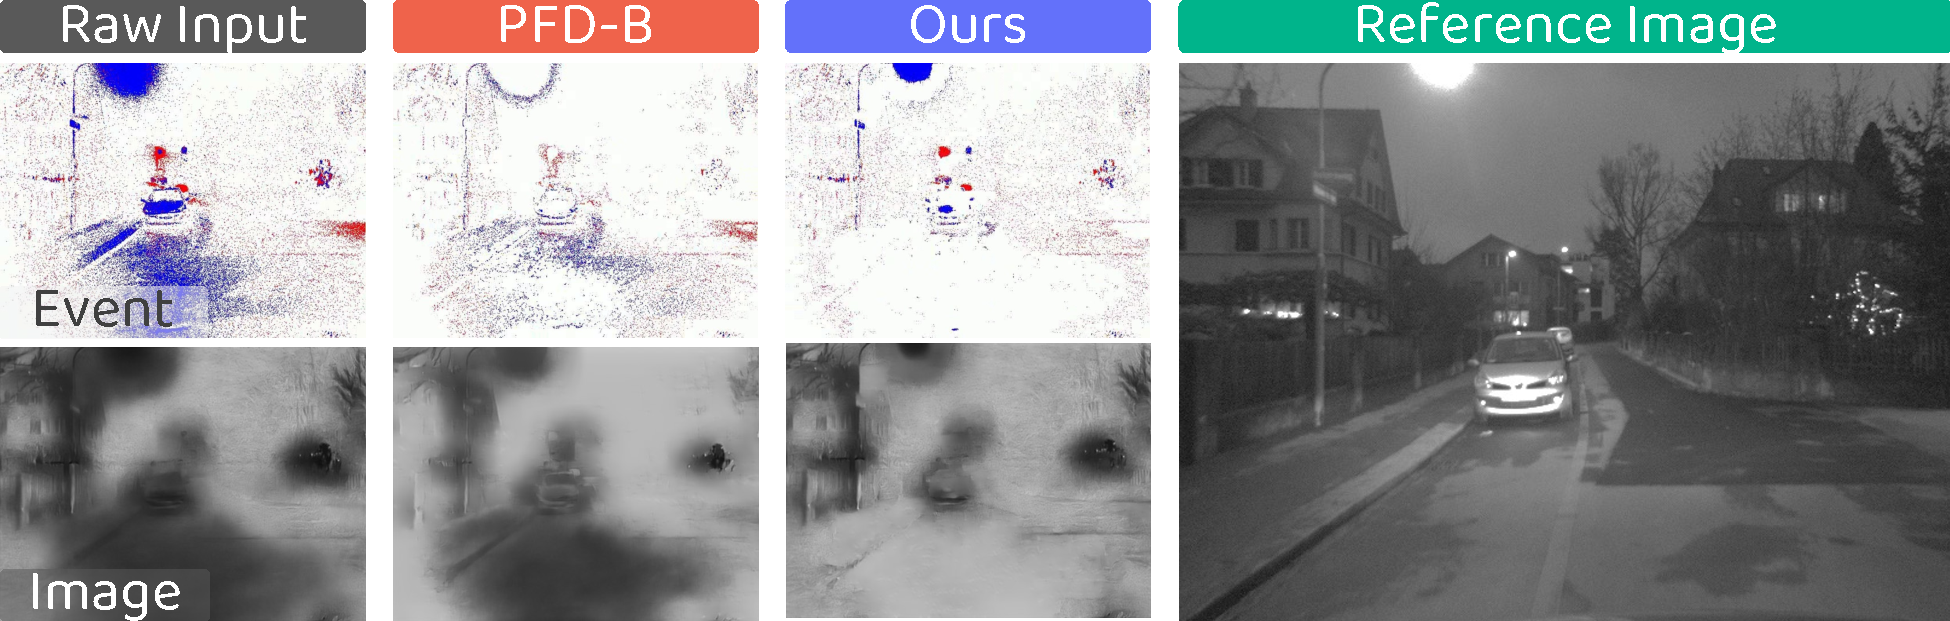
\includegraphics[width=\columnwidth]{figures/image_reconstruction.pdf}
    \vspace{-0.65cm}
    \caption{\textbf{Downstream task comparisons} for event-based imaging. We use SPADE-E2VID~\cite{cadena2021spade} to reconstruct images from both raw and our de-flared event streams on a challenging DSEC scene.}
    \label{fig:image_reconstruction}
    \vspace{-0.1cm}
\end{figure}
Collectively, these ablations confirm that the success of \textbf{E-Deflare} arises from principled physical modeling: (1) maintaining correct light source semantics in training targets, and (2) implementing the non-linear event suppression mechanism derived from the irradiance-domain interaction model.


\begin{table*}[t]
    \centering
    \caption{\textbf{Ablation study on the E-Flare-R dataset}. We evaluate three variants to analyze our core design choices. The final row shows the improvement of our full model over the best ablated variant ($\downarrow$: lower is better, $\uparrow$: higher is better). Ch. = Chamfer Distance; Gau. = Gaussian Distance; PM2/PM4 = Pooled MSE at scales 2/4.}
    \vspace{-0.3cm}
    \label{tab:ablation_main}
    \small
    \resizebox{\textwidth}{!}{%
    \begin{tabular}{lcccccccc}
    \toprule
    \textbf{Config.} & ~~Ch.$\downarrow$~~ & ~~Gau.$\downarrow$~~ & ~MSE$\downarrow$~ & ~PM2$\downarrow$~ & ~PM4$\downarrow$~ & ~R-F1$\uparrow$~ & ~T-F1$\uparrow$~ & ~TP-F1$\uparrow$~
    \\
    \midrule
    \textcolor{gray}{$\bullet$}~\textcolor{gray}{Raw Input} & \cellcolor{gray!20}\textcolor{gray}{$1.7855$} & \cellcolor{gray!20}\textcolor{gray}{$0.7170$} & \cellcolor{gray!20}\textcolor{gray}{$0.8158$} & \cellcolor{gray!20}\textcolor{gray}{$0.3431$} & \cellcolor{gray!20}\textcolor{gray}{$0.3266$} & \cellcolor{gray!20}\textcolor{gray}{$0.2299$} & \cellcolor{gray!20}\textcolor{gray}{$0.2915$} & \cellcolor{gray!20}\textcolor{gray}{$0.3093$}
    \\\midrule
    \textcolor{ev_green}{$\bullet$}~No Light & $1.9745$ & $0.8487$ & $0.1951$ & $0.0843$ & $0.0806$ & $0.0189$ & $0.0459$ & $0.0709$
    \\
    \textcolor{ev_red}{$\bullet$}~Simple & \cellcolor{ev_red!20}$1.3434$ & \cellcolor{ev_red!20}$0.5564$ & \cellcolor{ev_red!20}$0.1816$ & \cellcolor{ev_red!20}$0.0734$ & \cellcolor{ev_red!20}$0.0688$ & \cellcolor{ev_red!20}$0.2703$ & \cellcolor{ev_red!20}$0.2768$ & \cellcolor{ev_red!20}$0.2644$
    \\
    % \textcolor{ev_red}{$\bullet$}~Full Model $+$ Jitter & $1.6811$ & $0.7203$ & $0.2020$ & $0.0834$ & $0.0788$ & $0.1567$ & $0.2001$ & $0.2103$
    % \\
    \midrule
    \textcolor{ev_blue}{$\bullet$}~\textbf{Full Model (Ours)} & \cellcolor{ev_blue!20}$\mathbf{1.1368}$ & \cellcolor{ev_blue!20}$\mathbf{0.4651}$ & \cellcolor{ev_blue!20}$\mathbf{0.1741}$ & \cellcolor{ev_blue!20}$\mathbf{0.0690}$ & \cellcolor{ev_blue!20}$\mathbf{0.0644}$ & \cellcolor{ev_blue!20}$\mathbf{0.3498}$ & \cellcolor{ev_blue!20}$\mathbf{0.3386}$ & \cellcolor{ev_blue!20}$\mathbf{0.3011}$
    \\
    \emph{Improvement (\%)} $\uparrow$ & $15.4\%$$\uparrow$ & $16.4\%$$\uparrow$ & $4.1\%$$\uparrow$ & $6.0\%$$\uparrow$ & $6.4\%$$\uparrow$ & $29.4\%$$\uparrow$ & $22.3\%$$\uparrow$ & $13.9\%$$\uparrow$
    \\
    \bottomrule
    \end{tabular}%
    }%
\vspace{-0.2cm}
\end{table*}



\subsection{Downstream Task Evaluations}
\label{sec:downstream}

To validate the generalizability of our framework, we evaluate \textbf{E-Deflare} on two high-level tasks: image reconstruction and 3D scene reconstruction.


\begin{table}[t]
    \centering
    \caption{\textbf{Downstream task comparisons} for event-based 3D reconstruction. We use Event3DGS~\cite{han2024event} to reconstruct scenes and evaluate the quality of novel view synthesis. $\uparrow$: higher is better.}
    \label{tab:3dgs_quant}
    \small
    \resizebox{\columnwidth}{!}{%
    \begin{tabular}{r|c|ccc|c}
    \toprule
    \textbf{Metric} & \textcolor{gray}{Original} & EFR & PFD-A & PFD-B & \textbf{Ours}
    \\
    \midrule
    PSNR $\uparrow$ & \cellcolor{gray!20}\textcolor{gray}{$13.72$} & \cellcolor{ev_red!20}$13.74$ & $13.11$ & $13.32$ & \cellcolor{ev_blue!20}$\mathbf{13.78}$
    \\
    SSIM $\uparrow$ & \cellcolor{gray!20}\textcolor{gray}{$0.765$} & $0.741$ & \cellcolor{ev_red!20}$0.743$ & $0.734$ & \cellcolor{ev_blue!20}$\mathbf{0.792}$
    \\
    \bottomrule
    \end{tabular}}
    \vspace{-0.1cm}
\end{table}
\noindent\textbf{Event-based Imaging.}
We first assess the impact of de-flaring on event-to-image reconstruction using the state-of-the-art SPADE-E2VID framework~\cite{cadena2021spade}. Fig.~\ref{fig:image_reconstruction} shows results on challenging sequences in \textbf{DSEC-Flare}. Images reconstructed from raw, flare-corrupted events exhibit strong flare patterns, obscuring fine scene details. In contrast, images reconstructed from our de-flared events recover cleaner and accurate illumination, revealing significant visual improvement. These results demonstrate that \textbf{E-Deflare} serves as an effective pre-processing step, substantially enhancing the clarity and usability of event data for imaging applications.




% \noindent\textbf{Event-based 3D Reconstruction.}
% To demonstrate the practical impact of our method, we conduct a rigorous quantitative evaluation on the downstream task of event-based 3D reconstruction. As no standard benchmark with flare artifacts exists for this task, we created one by synthesizing paired event datasets using the popular LEGO scene from the NeRF-synthetic \cite{mildenhall2021nerf} dataset, following the simulation methodology of PECS \cite{han2024physical}.

% Using the method from Event3DGS~\cite{han2024event}, we reconstruct a 3D scene from the original flare-corrupted input, our de-flared output, and the outputs from baseline methods. We then evaluate the quality of each reconstruction by rendering novel views and comparing them against the pristine ground truth. To ensure fairness, the background is color-normalized during metric calculation.

% The results in Table~\ref{tab:3dgs_quant} reveal that naive de-flaring can be detrimental. Most baselines fail to improve reconstruction, with some even degrading performance below the original input. In stark contrast, our method is the only one to provide a clear and consistent improvement, boosting the SSIM from $0.765$ to a state-of-the-art $\mathbf{0.792}$ where all others falter. This powerfully demonstrates that our approach provides a cleaner, more reliable input that directly benefits downstream 3D perception.

\noindent\textbf{Event-based 3D Reconstruction.}
To demonstrate the practical impact of our method, we conduct a rigorous quantitative evaluation on event-based 3D reconstruction. As no standard benchmark with flare artifacts exists for this task, we synthesized a paired event dataset from the popular LEGO scene of NeRF-synthetic~\cite{mildenhall2021nerf}, following the simulation methodology of PECS~\cite{han2024physical}. The experimental process involves reconstructing a 3D scene from various event streams (the original flare-corrupted input, our de-flared output, and outputs from baseline methods) using Event3DGS~\cite{han2024event}. We then evaluate the reconstruction by rendering novel views and comparing them against the pristine ground truth, with background color normalization for a fair comparison.



\begin{figure}[t]
    \centering
    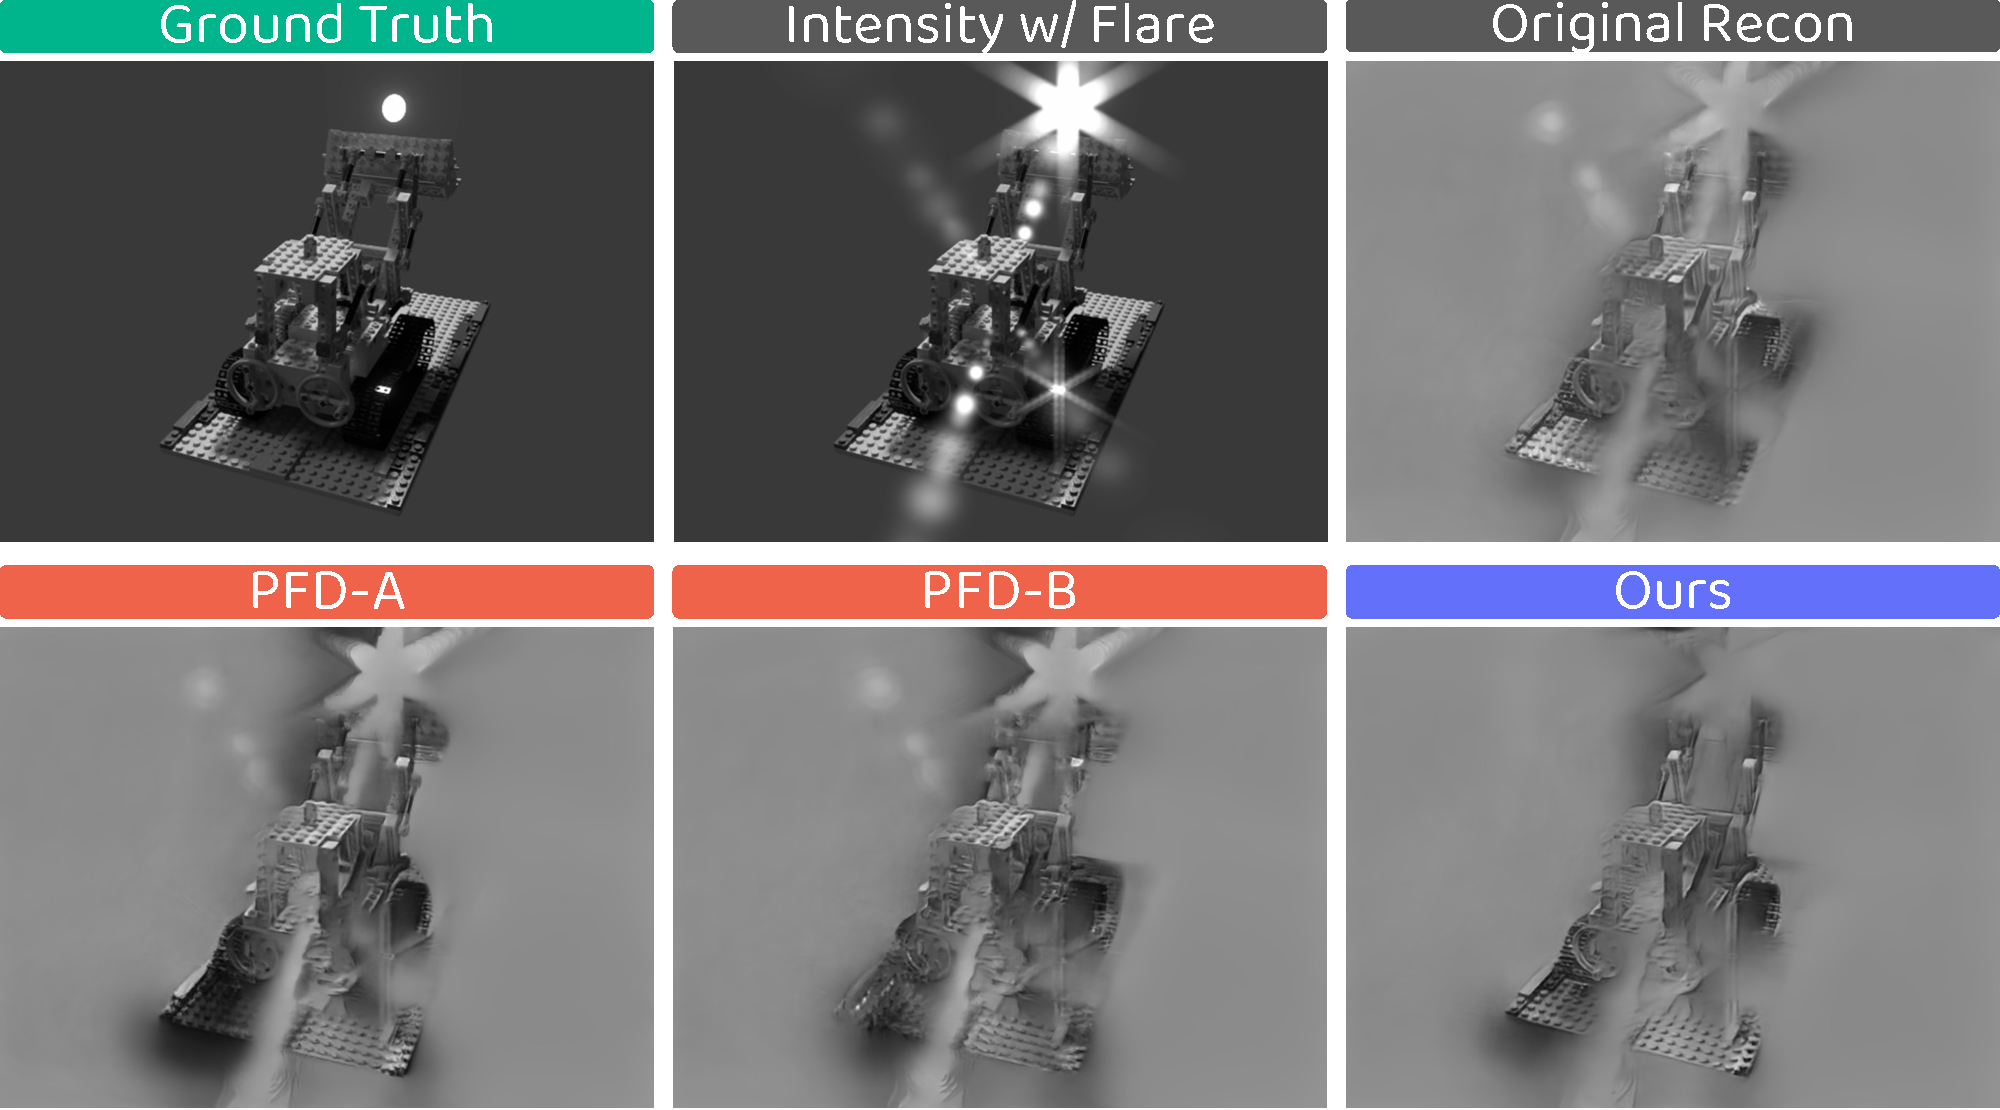
\includegraphics[width=\columnwidth]{figures/3D_reconstruction.pdf}
    \vspace{-0.65cm}
    \caption{\textbf{Downstream task comparisons} for event-based 3D reconstruction. We visualize the rendered views from 3D scenes reconstructed using the outputs of different de-flaring methods.}
    \label{fig:3dgs_qual}
    \vspace{-0.1cm}
\end{figure}
The results in Table~\ref{tab:3dgs_quant} reveal that naive de-flaring can be detrimental. Most baselines fail to improve reconstruction, with some even degrading performance below the original input. In contrast, our method is the only one providing a clear and consistent improvement, boosting the SSIM from $0.765$ to a state-of-the-art $\mathbf{0.792}$. This powerfully demonstrates that our approach provides a cleaner, more reliable input that directly and substantially benefits downstream 3D perception tasks.


%old version, the bg have different color

% % --- Table for 3D Reconstruction ---
% \begin{table}[t]
%     \centering
%     \caption{Quantitative results for the downstream task of event-based 3D reconstruction. Our method leads to higher quality novel view synthesis, evaluated by PSNR, SSIM, and LPIPS metrics.}
%     \label{tab:3dgs_quant}
%     \small
%     % The 'booktabs' package is needed for \toprule, \midrule, \bottomrule
%     \begin{tabular*}{\columnwidth}{l@{\extracolsep{\fill}}ccccc}
%     \toprule
%     Metric & Original & EFR & PFD-A & PFD-B & \textbf{Ours} \\
%     \midrule
%     PSNR $\uparrow$ & 14.29 & 14.22 & 13.67 & 13.92 & \textbf{14.32} \\
%     SSIM $\uparrow$      & 0.759 & 0.747 & 0.735 & 0.739 & \textbf{0.777} \\
%     LPIPS $\downarrow$   & \textbf{0.273} & 0.308 & 0.287 & 0.298 & 0.285 \\
%     \bottomrule
%     \end{tabular*}
% \end{table}
